\newcommand{\freeprocessing}[0]{\textit{Free}processing}
\newcommand{\freeprocessor}[0]{\textit{free}processor}
\newcommand{\nullset}[0]{$\varnothing$}
\newcommand{\insitu}[0]{\textit{in situ}}

%\newcommand{\nullset}[0]{$\emptyset$}
\definecolor{lightgray}{gray}{0.85}

\textit{In situ} visualization has become a popular method for avoiding
the slowest component of many visualization pipelines: reading data
from disk.  Most previous \insitu{} work has focused on achieving
visualization scalability on par with simulation codes, or on the data
movement concerns that become prevalent at extreme scales.
In this work, we consider \insitu{} analysis with respect to ease of
use and programmability.  We describe an abstraction that
opens up new applications for \insitu{} visualization, and demonstrate
that this abstraction and an expanded set of use cases can be realized
without a performance cost.

\section{Introduction and related work}

% The growing size of simulation outputs
% - sims producing much more data
% - too slow to load in for vis
% -> rise of in situ
% - other approaches as well
%   - data staging (io nodes)
%     - enables asynch
%   - co-analysis
%   - acceleration of io (vishwanath)

The growing size of simulation data and the problems this poses
for subsequent analysis pipelines has driven simulation authors to
integrate visualization and analysis tasks into the simulation
itself~\cite{Childs:2013:ChallengesVis}.  The primary advantage of
this approach is to perform operations on data while they are still in
memory, rather than forcing them through disk, thereby eliminating the
most expensive component of the majority of visualization and analysis
pipelines.

Scientists and engineers have developed many different approaches
to \insitu{}.  DART uses RDMA to stage data from supercomputer to
potentially separate analysis-focused
resources~\cite{Docan:2010:DART}, and a system performs computations on
the data as they are in transit from one resource to
another~\cite{Moreland:2011:InTransit}.  The dominant approach is
to use the same supercomputer that is running the simulation for
visualization, though potentially on just a subset of cores, in the
manner of
Damaris/Viz~\cite{Dorier:2013:Damaris}.  Damaris/Viz can provide a
wealth of visualization and analysis opportunities due to its ability
to act as a
front end to both VisIt's~\cite{Childs:2012:VisIt}
\texttt{libsim}~\cite{Whitlock:2011:Libsim} as well as ParaView's
Catalyst~\cite{Fabian:2011:Catalyst, CatalystUserGuide}.  Biddiscombe
et al. proposed an HDF5-based driver that forwards the data from HDF5
calls to ParaView~\cite{Biddiscombe:2011:HDF5Steering}; we give an
example of our system implementing similar functionality in
\S~\ref{sec:enzo-example}.  Abbasi et al. introduce DataStager,
a system for streaming data to staging nodes and demonstrate a
performance benefit by asynchronously streaming multiple buffers at one
time~\cite{Abbasi:2009:DataStager}. \textit{In situ} libraries can also
be used to improve the performance of simulation
code~\cite{Vishwanath:2011:Leadership}.

Most work focuses on extreme-scale performance with less regard for the
effort required in integrating simulation and visualization software,
whereas we focus on the latter concern.  Notably, however, Abbasi et
al. extend their previous work with a JIT compiler that allows users to
customize data coming through
ADIOS~\cite{Lofstead:2008:ADIOS} using snippets of code written in a
subset of
C~\cite{Abbasi:2011:JITStaging}.  Zheng et al. modify OpenMP runtimes,
an approach that shares our mentality of working within the
constraints of existing
infrastructure~\cite{Zheng:2013:GoldRush}.  Others have tightly
integrated simulation with visualization to allow steering, but these
generally come at high integration costs~\cite{Lesage:2012:FlowSitu,
Ament:2011:Steering}.

% Freeprocessing can implement that idea for specific domains; the main
% differences are that binary instrumentation can do this with 1) any
% software and 2) for any writes, not just writes that go through a
% specific library.

% - existing solutions leave potential users behind
%   - difficulty / lack of desire for middleware
%   - maybe file i/o isn't synchronous (e.g. adios requires synchronous opens)
%   - perceived benefit (correct or no) too low
%   - existing infrastructure with custom domains

Existing solutions leave a potentially large segment of the user
community behind.  Most previous work has integrated or presupposed
integration with particular libraries for performing I/O operations,
and no such library has achieved universal adoption.
Yu et al. note the tight collaboration required
for a fruitful integration~\cite{Yu:2010:Combustion}.  Reasons for
not adopting I/O middleware are varied: the difficulty in integrating
the library with local tools, perceived lack of benefit, lack of
support for existing infrastructure with home-grown formats, or issues
conforming to required interfaces, such as synchronous `open' calls.

%   - simple problem/code: no need for middleware
%     - all the serial sims out there
%     - matlab / octave?
%   - middleware doesn't make any sense: HDF5 in openssh?
%   - additional libraries complicate code: must evolve together
%   - diverse use case
%     - non-simulation uses: provenance? instrument all launched programs

Moreover, the focus of modern I/O middleware specifically on
simulations at the extreme scale leaves a long tail of potential
\insitu{} uses behind.  The set of simulation authors focused on
creating exascale-capable simulations is a small subset of all
simulation authors.  A large set does not even dream of petascale;
and even larger are those who would barely know how to exploit a
terascale-capable solver for their science.  The distribution gets
larger and more diverse as one moves out to lower scalability levels.

At the opposite end of `extreme scalability' uses for \insitu{}, one
may find a number of heretofore ignored applications.  There is no
reason to limit the \insitu{} idea to parallel code running on a
supercomputer, for example.  Analysis routines embedded into the fabric
of network transfer operations would be a boon to distributed research
groups (and
the success of tools such as Globus~\cite{Foster:2011:Globus} speaks
to the multitudes of domains faced with this problem).  Those
writing simulations in MATLAB\textsuperscript{{\tiny \textregistered{}}} might
also benefit from precanned visualization tasks that occur concurrently
with their simulation, yet the closed source nature of the product
makes the prospect of integrating I/O middleware improbable at best.

The currently-dominant middleware approach to \insitu{} requires
significant effort.  It is reasonable for simulation authors to spend a
week integrating and retooling their code to achieve
thousand-way concurrent \insitu{} visualization, but this level of
investment is unreasonable to users who simply wants to compute a
data range on their files as they move across the country.  The cliff
between `nothing' and
a `100\%' solution for \insitu{} visualization with
existing middleware solutions is too high to appease such diverse
use cases.  Worse, the model is unworkable in some situations;
it is doubtful that the OpenSSH maintainers would accept patches
incorporating
ParaView's Catalyst into \texttt{sftp}, for example.

\textit{Free}processing is an abstraction of previous work.  Using
it, one can implement classical \insitu{} visualization and analysis,
computation or data reduction via staging nodes, unique instrumentation
such as gathering power consumption information
dynamically~\cite{Gamell:2013:InSituPower}, or a number of novel
`processing while moving data' ideas.  This processing can be
synchronous or asynchronous depending on the needs and desires of the
user.  Developers of a \freeprocessor{} can connect it to existing
visualization tools such as VisIt's \texttt{libsim} or ParaView's
Catalyst, implement their own analysis routines, and even push data
into another language such as Python, all without data
copying---\emph{or} with data copying, should those semantics be
preferable.  The general
nature of \freeprocessing{} not only allows one to implement the
diverse domains of previous work, but also allows novel use cases.
Specifically, we contribute:

% - freeprocessing is an abstraction of previous work
%   - can copy data or work with it in the same address space
%   - can be synchronous or asynchronous with simulation code
%   - can implement classical in situ
%   - can implement the `in transit' mode of DataStager
%   - can implement `DART'
%   - can implement visualization during data transfer
%   - can implement data conversion
%   - can forward data to ParaView's catalyst for tool-specific in situ
%   - can implement i/o acceleration (delayed closes?)
%   - can implement special provenance tracker

\begin{itemize}

  \item a new method for inserting data processing code into I/O
  operations;
%, including demonstrations that previous work can be
%  implemented within it;

  \item the generalization of \insitu{} ideas to heretofore unexplored
  domains, such as visualization during network transfer;

  \item greatly increased programmability for \insitu{} ideas, making
  them applicable with considerably less effort;

  \item a sample implementation that demonstrates all of these ideas in
  real-world cases.

\end{itemize}

The rest of this paper is organized as follows.  First, we explain the
technical underpinnings of how the program works.  In
\S~\ref{sec:classical} we demonstrate
\freeprocessing{} in some classical environments and show that there
is almost no overhead.  We demonstrate some novel uses
before we conclude and note limitations as well as future work in
\S~\ref{sec:fp-conclusion}.

% \section{Previous work}
%
% Others have proposed solutions to the problems within \insitu{}
% parallel visualization and analysis.

% Gamell et al. detail the power requirements of a prototypical \insitu{}
% workflow~\cite{Gamell:2013:InSituPower}.  DART uses RDMA to stage data
% from the supercomputer to potentially-separate
% analysis-focused resources~\cite{Docan:2010:DART}.  Continuing this
% idea of utilizing a smaller set of nodes for visualization and
% analysis, Damaris/Viz adds visualization to an I/O-oriented framework
% at demonstrably low
% overheads~\cite{Dorier:2013:Damaris}.  It can act as a frontend to
% both VisIt's~\cite{Childs:2012:VisIt}
% \texttt{libsim}~\cite{Whitlock:2011:Libsim} as well as
% ParaView's Catalyst~\cite{Fabian:2011:Catalyst}.  Biddiscombe et al.
% proposed an HDF5-based driver that forwards the data from HDF5 calls
% to ParaView~\cite{Biddiscombe:2011:HDF5Steering};
% \S~\ref{sec:enzo-example} gives an example of our system implementing
% similar functionality.

% In doing so, we make simulation software easier to instrument, make it
% much simpler to plug-in alternate visualization and analysis tools, and
% enable uses of `\insitu' ideas in novel environments.

% [in contrast to GoldRush], our method 1) requires no maintenance for
% updating runtimes, 2) works even if a simulation does not utilize
% OpenMP, and 3) does not have the initial cost of porting to a new
% runtime.

% \section{Structure of a simulation}
%
% The common method to enable \insitu{} visualization in an existing
% simulation is to make a coupling library available to simulation
% software, change the simulation source code to call the new API, and
% recompile the simulation code, additionally linking the visualization
% tool as a library.  This is a significant investment: while the
% multiple simulations that use it can amortize the development costs
% of the coupling library, instrumenting the simulation source code
% is necessarily a per-simulation cost.  Furthermore, visualization
% software is typically multiple orders of magnitude more complicated
% to build than the simulation code that then utilizes it.  This
% can be a large barrier, particularly when simulation authors are
% not well-versed in the arcane lore of large-scale C++ software
% development.
%
% One of the most complicated components of this process is in
% modifying the simulation code: it must push the data over to the
% visualization software, and it must relinquish and regain control
% periodically to allow the visualization tool to produce its output.
% The decision of where to insert these code changes can be difficult
% for a simulation author, especially when the simulation scales better
% than the visualization tool.  Insertion of this `glue' code is also
% problematic if there are cases in which running the visualization
% tool is undesirable or even impossible---for example, when the
% simulation tool supports a particular esoteric architecture that the
% visualization tool does not.  Furthermore, there can be an impedance
% mismatch between the two tools, for example if the visualization tool
% requires both a grid and associated data in a single call, but the
% simulation does not colocate this information in time (instructions)
% or space (memory).
%
% Yet all simulations must fulfill the contract of writing and
% describing its data, at some point.  To this end, we have analyzed
% a number of simulation packages to identify their overall
% structure---essentially the operations in their outermost loops.

\section{Instrumentation}
\label{sec:instrumentation}

\begin{figure*}
  \centering
  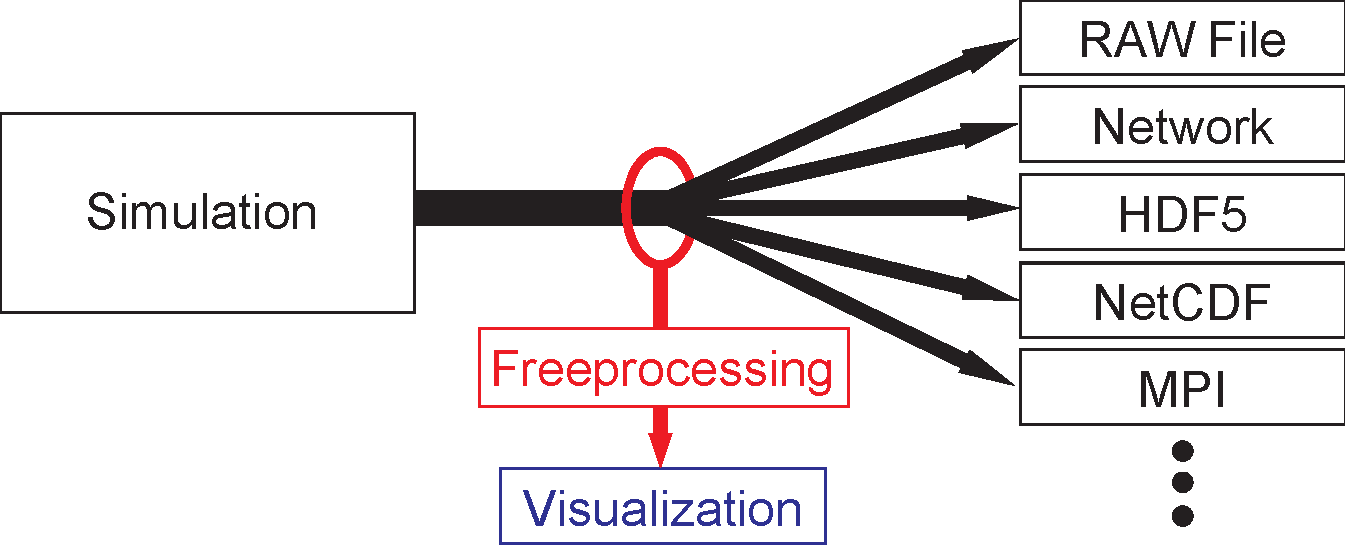
\includegraphics[width=0.95\linewidth]{images/fp/fp}
  \caption{\textit{Free}processing works like a vampire tap on the data
  coming out of a simulation.  Without changes to a program's source
  code, we can intercept the data as it goes to the IO library and
  inject visualization and analysis tasks.}
  \label{fig:interchange}
\end{figure*}

Previous \insitu{} solutions have relied on the simulation author
explicitly invoking the visualization tool, or the simulation using a
custom library for I/O that is then repurposed for analysis.  In this
work we demonstrate that there is little need for
either; every simulation produces output already, an \insitu{} tool
just needs to tap into that output.

Our symbiont uses binary instrumentation to realize that tap. We take
unmodified simulation binaries and imbue them with the ability to
perform visualization and analysis tasks.  In doing so, we remove a
potentially
complicated component of \insitu{}: modifying the program to work with
the visualization or analysis tool.  Notably, this approach
enables simulation software to produce \insitu{} visualizations even
when the source code of the simulation is unavailable.  Furthermore, as
the symbiont interposes these functions during load time, a user need
only change the invocation of the program to enable or disable these
features.

%%%% ---- %%%%%

The method we use is to redefine some of the standard I/O functions, in
a similar manner to the way the
GLuRay or Chromium systems operate~\cite{Brownlee:2012:GLuRay,
Humphreys:2002:Chromium}.  These methods rely on features available in
runtime dynamic linkers to replace any function implemented within a
library at load time.  The overridden entry points form what we call
the `symbiont', the core of
\freeprocessing{}. The symbiont's purpose is to conditionally forward
data to a
\freeprocessor{}---a loadable module that implements the
desired \insitu{} computation---in addition to fulfilling the
function's original duties.  Separating the instrumentation itself and
the \freeprocessor{} allows users to develop processing elements
without knowledge of binary instrumentation.

The set of intercepted functions is different depending on the I/O
interface that the
simulation uses, as shown in Figure~\ref{fig:interchange}.  For the C
language, these functions are those of the POSIX
IO layer, such as \texttt{open(2)} and \texttt{write(2)}.  In Fortran
these calls are implementation-specific, and C++ implements I/O
differently, but on POSIX-compliant systems all such implementations
are ultimately layered on top of the POSIX I/O interface.  We also
introduce interposition for higher-level functions, such as those that
comprise MPI File I/O, and a subset of calls from the HDF5 family.
Using this interposition, what the simulation believes is a standard
`write' operation actually calls in to our symbiont.

\subsection{Data semantics}

Function interposition for higher-level functions from libraries such
as HDF5 and NetCDF provide an important benefit: data semantics.  As
these formats are self-describing, there is enough information in just
the stream of function calls to identify data properties---in contrast
to raw POSIX I/O functions that provide little more than an abstract
buffer.  The symbiont forwards any available data semantics from the
interposed library functions to the
\freeprocessor{}.

However, in contrast to previous work, \freeprocessing{} will also
willingly forward data without knowledge of any underlying semantics.
A \freeprocessor{} can also ignore metadata simply by not implementing
the methods that interpret those messages.  This distinction is
important, as it both enables \freeprocessing{} to function in a larger
set of scenarios, as well as increases the flexibility of the system.
Presumably a \freeprocessor{} would then obtain this information from
some external source.  We view allowing semantic-less data transfer
similar to using `dangerous' constructs in a programming language, such
as casts in C.  While these constructs are generally
frowned upon, with restrained application they can be a powerful and
thereby useful tool.

% We view it much in the same way as a cast in C: it is dangerous,
% unwieldy, and a source of bugs, so one should never program this
% way---unless, of course, you have to, or it would be really inefficient
% otherwise, or it is an
% hour before a meeting and you \emph{need} this result, or these data
% really \emph{will always} be $32^3$, or ...

\subsection{Data semantics}

Meta-information concerning data semantics are required, and are
only available through \freeprocessing{} in limited cases.  While we
consider such concerns beyond the scope of this work, they need to be
provided for the demonstration of the technique.  The general nature of
\freeprocessing{} allows any number of solutions: the problem is no
different than understanding arbitrary binary data read from a file.
One of the solutions we have found works well is a simple text file
in the style of Damaris/Viz or ADIOS~\cite{Dorier:2013:Damaris,
Lofstead:2008:ADIOS}.  An example of one such configuration
is given in Listing~\ref{lst:jscfg}.  However, it is important to
note that this configuration is external to \freeprocessing{}
itself.  The symbiont does not contain this parsing and metadata
acquisition code; the `user
code'---\freeprocessor{}s---implements this only if they desire.

%We provide code that the user can drop into their code for this
%purpose, but there is no library a user must link against to implement
%a
%\freeprocessor{}.  Not forcing a metadata mechanism is useful, for
%example, in the instrumentation of PsiPhi (\S~\ref{sec:psiphi}), which
%already describes its output in a custom manner.  In previous work, such
%metadata would need to be duplicated in the \insitu{} tool's
%configuration.

\begin{minipage}{\linewidth}
\lstinputlisting[label=lst:jscfg,caption=JSON configuration file used
for a Silo conversion \freeprocessor{}.  Variants that do not require
the repeated \texttt{"i"}s are possible\textrm{,} but lack the desirable
property of strict adherence to the JSON specification.]{silo.json}
\vspace{-0.01em}
\end{minipage}

\freeprocessing{} itself does not endorse any specific method for
obtaining data semantics, in the same way that the C file I/O routines
do not endorse a specific encoding for metadata on binary streams.

%We note, however, that \freeprocessing{} leaves issues related to data
%semantics open.  There are a plethora of methods to communicate this
%information out-of-band, all of which are possible to implement with
%\freeprocessing.

\subsection{Defining \freeprocessor{}s}

The module interface for a \freeprocessor{} is simple.  The system
exposes a stream processing model.  Data are input to the processor,
utilized (or ignored), and thereafter unavailable.  This interface is
in principle the same model as GLSL, OpenCL, and CUDA expose, though we do not
currently impose the same restrictions.  A \freeprocessor{} is free to
implement a cache and process data in a more traditional manner, for
example.

Listing~\ref{lst:interface} shows the \freeprocessor{} interface.
The symbiont calls \texttt{Init} when a file is first accessed; some of
our \freeprocessor{}s initialize internal resources here.  The
\texttt{filename} parameter allows the processor to provide different
behavior should the simulation output multiple file formats.  The
\texttt{buffer} and \texttt{n} parameters are the data and its size in
bytes.  If the required information is available, the symbiont will call
\texttt{Metadata} immediately before a write, communicating the
characteristics for the impending data.  Likewise,
\texttt{finish} cleans up
any per-file resources.  Finally, the \texttt{create} function
implements a `virtual constructor' to create the processor.
All functions sans \texttt{create} are optional; if a
\freeprocessor{} has no need for metadata, for example, it simply does
not implement the corresponding function.

\begin{minipage}{\linewidth}
\lstinputlisting[language=C++,label=lst:interface,caption=Base class for a
\freeprocessor{}.]{interface.c}
\vspace{-0.01em}
\end{minipage}

\subsubsection{Configuration}

The symbiont reads a configuration file that describes
which \freeprocessor{}
to execute.  Any library that satisfies the interface given in
Table~\ref{lst:interface} is a valid \freeprocessor{}.  It is important
to note that the operations share the semantics of the simulation code.
For example, if a parallel simulation performs only collective writes
for a given file, then it is appropriate to perform
collective operations in the \freeprocessor{}'s \texttt{Stream} call.

It is common for a simulation to produce a large set of output
files.  Furthermore, MPI runtimes frequently open a number of files
to configure their environment, and all these files are `seen' by the
symbiont.  It is therefore necessary to provide a number of filtering
options.  Some of these are built in, such as ignoring files that
are opened for read-only access.  Others the user specifies in the
configuration file for the symbiont.  The specification uses a match
expression for the filenames, so the user can further limit where
instrumentation will occur.  These match expressions provide a more
convenient mechanism to uniquely connect processing elements to
streams, but the
assignment could also be done by the \freeprocessor{} implementation.

\subsubsection{Python}
\label{sec:python}

Developers may also implement \freeprocessor{}s in Python.  We provide a simple
\freeprocessor{} that embeds the Python interpreter and exports data
and needed metadata.  Most notably, it creates the
`\texttt{stream}' variable: a NumPy array for the data currently being
written.  Exposing the array to Python does not require a copy; the
simulation data shares the memory with the Python runtime.  Should
the Python script attempt any write operation on the data, a copy is
transparently made inside the Python runtime that is then managed via
Python's garbage collector.  We allow only one of the simulation or the
Python tool to run at any given time.

The Python script is otherwise indistinguishable from standard Python
code; the symbiont imposes no restrictions beyond the unique source of
data.  Communication via, e.g., MPI4Py is even possible, provided the
simulation utilizes synchronous writes.
In \S~\ref{sec:enzo-example} we demonstrate this method by connecting
\freeprocessing{} with the \texttt{yt}
visualization tool~\cite{Turk:2010:yt}.

% It is worth noting that choosing to utilize Python somewhat complicates
% the use of \freeprocessing{}.  In particular, search paths for Python
% libraries---and shared libraries they link against---must be carefully
% configured so that they propagate into the more limited environment of
% the simulation code.  This is no different than the situation with, for
% example, ParaView's Catalyst; their documentation notes the same
% tradeoff~\cite{CatalystUserGuide}.

\section{Classical in situ}
\label{sec:classical}

\freeprocessing{} can implement a number of \insitu{} ideas,
including the traditional use case of \textit{in situ}: visualization
and analysis during a simulation run.  In this section, we detail how
the
corresponding \freeprocessor{}s for a few simulation codes operate, and
demonstrate that the overhead of the method is negligible.

\subsection{PsiPhi}
\label{sec:psiphi}

\begin{figure}
  \centering
  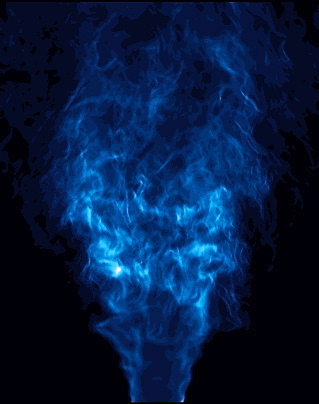
\includegraphics[width=0.48\linewidth]{images/fp/PsiPhi-vring.png}
  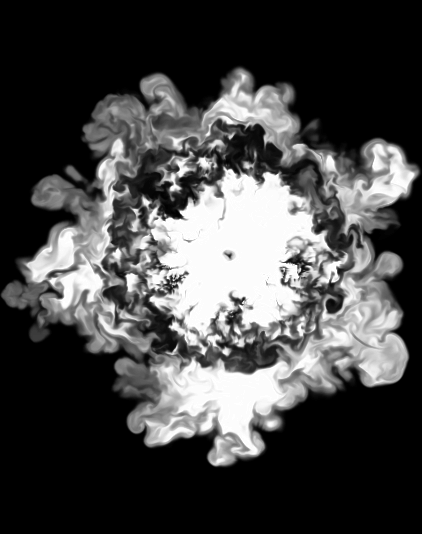
\includegraphics[width=0.48\linewidth]{images/fp/PsiPhi-slice.png}
  \caption{Sample \textit{in situ} visualizations of the Cambridge
  stratified flame produced by the PsiPhi code.}
  \label{fig:PsiPhi}
\end{figure}

PsiPhi is a Fortan95/2003-based CFD-solver that focuses on Large Eddy
Simulation (LES) of flows that include combustion and other types of
chemical reactions.  The simulation discretizes the governing equations
of mass, momentum, and species concentration on a cartesian grid via
the finite volume method.  Second-order schemes discretize the domain,
and an explicit third-order low storage Runge-Kutta scheme advances
the solution.  The immersed boundary (IB) technique handles diverse
geometries in a computationally efficient manner.  Besides the solution
of the mentioned transport equations in an Eulerian formulation, the
code is able to solve the equations of motion for Lagrangian particles.
A combination of Lagrangian particles and immersed boundaries describes
moving objects.  The code is modular, easy to extend and maintain, and
highly portable to different machines.  PsiPhi parallelizes via the
distributed-memory paradigm, using MPI.

% would be good if \cite{Franchetti2013PCI} fit in this list as well...

PsiPhi simulates highly-resolved simulations of reactive flows, e.g.,
premixed, non-premixed and stratified combustion, coal and biomass
combustion, liquid spray combustion, and nanoparticle
synthesis~\cite{Pettit2011PCI, Ma2013CTM, CavalloMarincola2013PCI}.
The software has scaled to thousands of cores on Top500 machines such
as SuperMUC and JUQUEEN.  Recent tests with the program have shown
that the output of the computational results becomes a performance
bottleneck when moving up to an even higher number of cores.

There are three types of intermediate outputs in the PsiPhi simulation.
The first
are actually custom-developed \textit{in situ} visualizations: slice
outputs and volume renderings.  The simulation writes out these
visualizations in custom ASCII-based formats every $n$ time steps, with
typical values of $n$ in
between 100 and 1000~\cite{Proch2014CNF};
Figure~\ref{fig:PsiPhi} shows example visualizations.  The second type
of output is a simulation-specific binary format used for restart files
that is organized in a `one file per process' manner.  Synchronous
Fortran `unformatted'
\texttt{WRITE} operations create these outputs.  The third kind of
output is an ASCII-based metadata file that describes the layout of the
binary restart files.

The PsiPhi authors are interested in extracting arbitrary 2D slices
as well as 3D visualizations with more flexibility than their
custom-developed routines allow.
Therefore, we developed a custom \freeprocessor{} for the PsiPhi
simulation.  PsiPhi periodically dumps its state to disk in the form
of restart files, at approximately the same cadence as `normal' output
files.  We utilized the aforementioned restart files as the basis for our
\freeprocessor{}, in addition to parsing the ASCII-based metadata to interpret
these restart files.

% As such, we elected to utilize these restart files as the basis
% for our \freeprocessor{}.  Fortunately, PsiPhi was also writing a
% simple ASCII file that described its fields, and so we glean the
% needed metadata from the writing of this file.

\begin{figure}
  \centering
  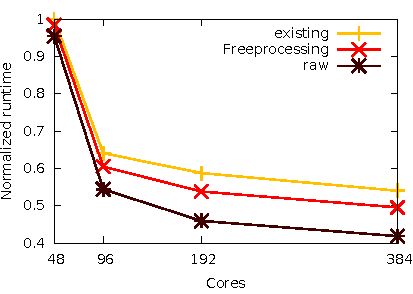
\includegraphics{images/fp/scaling.pdf}

  \caption{Scalability of the PsiPhi simulation. `existing' and
  `Freeprocessing' produce the same outputs via different mechanisms,
  while `raw' produces only restart files.  Freeprocessing's
  overhead is negligible; new output methodologies can even increase
  performance.}

  \label{fig:scaling}
\end{figure}

The simulation authors were enthusiastic about the
\freeprocessor{}.  All the outputs the simulation previously created
were redundant with the restart files.  Furthermore, PsiPhi users
hardcoded postprocessing parameters such as slice numbers into the
simulation source, necessitating a recompile to modify the parameters.
In light of the visualization
options presented by the \freeprocessor{}, the PsiPhi authors elected
to remove
all custom-developed \insitu{} outputs and create only the restart
files.

We therefore reimplemented their outputs in a \freeprocessor{} and
measured the performance of the system under both the old and new
configurations.  As
shown in Figure~\ref{fig:scaling}, not only was the overhead miniscule,
but the
simulation actually ran \emph{faster} with the \freeprocessor{}.  The
performance difference arose from the difference in how PsiPhi and
the \freeprocessor{} organize their writes.  In the
\freeprocessor{}, we calculate the appropriate file offsets on each
rank and output to a shared file directly; the original PsiPhi approach
was to gather the data on the root processor and then do all writing
from there.

% PsiPhi future:
%   specification of slices: *always* want mid-slice
%   want the same slices for every field; no need to change it per-field
%
%
% they typically take 2D slices, and then pull a line out from those
% slices. then they want to see an average (over time) and/or root
% mean square of the data along that line. compare it with a limited
% quantity of measured data. put it all together in gnuplot.
%
% they do this for a series of lines. often they take multiple slices
% and multiple lines.
%
% there is a desire to compare different simulations. done visually, or
% by putting the lines from different runs together in gnuplot.
%
% common workflow:
%
%   1. ssh to remote machine
%   2. run script to get the lines desired into PROFILE/ dir.
%   3. scp PROFILE/ dir to local machine
%   4. run another script to pull out line data into form for gnuplot
%
% this is painful.  would be nice if something could automate all that crap.
%
% desire single UI that knows all the machines you're using and can ssh to
% them and grok this information to display it.  in the end, want to see a
% slice and be able to drag and move it.

\subsection{Enzo}
\label{sec:enzo-example}

\begin{figure}
  \centering
  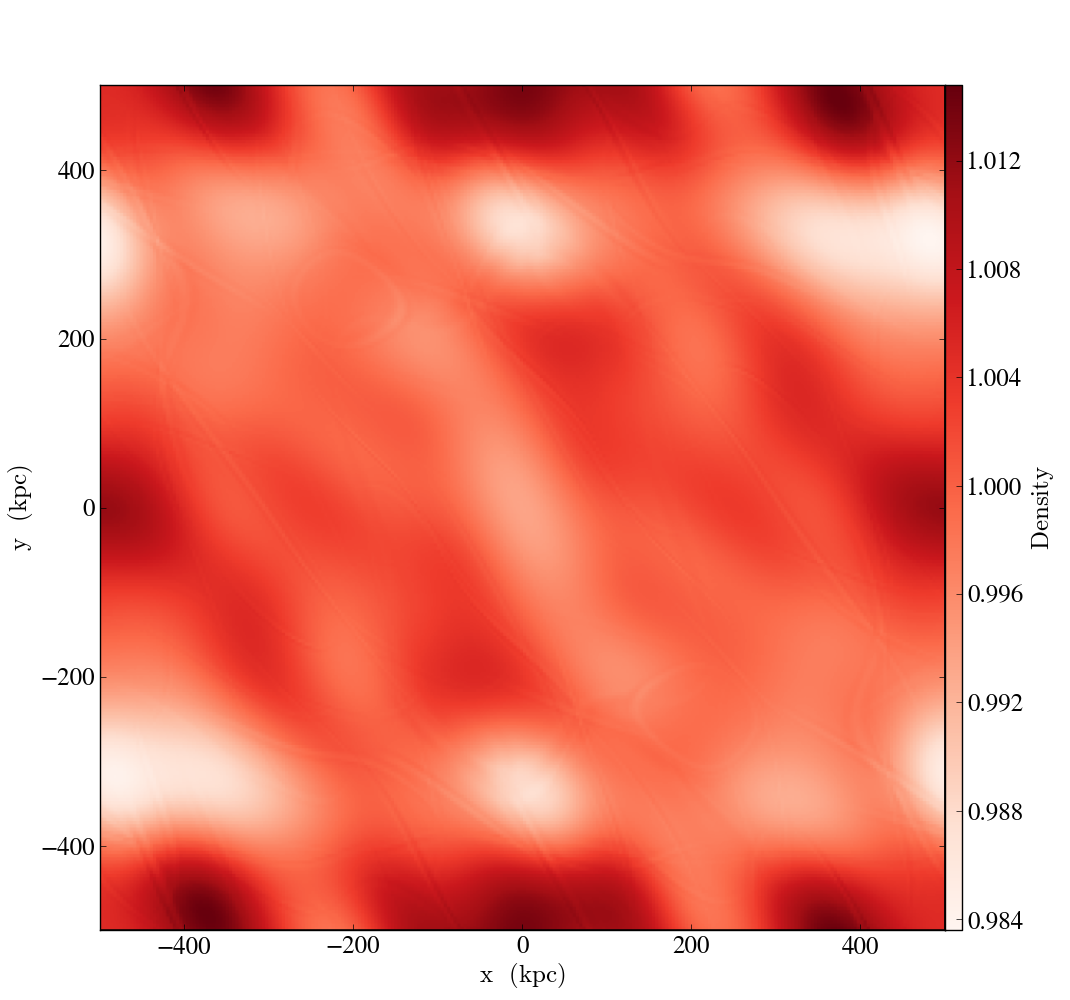
\includegraphics[width=\linewidth]{images/fp/enzo-density}
  \caption{`Density' field generated in situ by the Python
  visualization tool `yt' applied to an Enzo hydrodynamics simulation.
  A \freeprocessor{} exposed the data into Python and a standard yt
  script created the visualization.}
  \label{fig:enzo}
\end{figure}

Enzo is a simulation code designed for rich, multi-physics hydrodynamic
astrophysical calculations~\cite{Enzo:2013}.  It is of special interest
in the visualization community due to its use of adaptively-refined
(i.e., AMR) grids.  Enzo runs in parallel via MPI and CUDA on some of
the world's Top 500 supercomputers, with OpenMP hybrid parallelism
under investigation.  For I/O, Enzo relies on the HDF5 library.

As Enzo is HDF5-based and HDF5 provides all the data semantics
required, the selection of which fields are of interest is the only
required work.  For HDF5 outputs, the symbiont configuration file
specifies the `Datasets' (in the HDF5 sense) of interest as opposed to
a filename; the symbiont assumes that all HDF5 files opened for write
access are a simulation output.

When Enzo was first investigated, HDF5 support was not available in our
symbiont.  Generic HDF5 support in the symbiont required only a day of
effort.  Configuring it to work with Enzo takes seconds. Users must
edit a text file to indicate which field[s] they wish to see.  To work
with
Enzo's \texttt{yt} tool, we utilize the aforementioned
\freeprocessor{} that exposes data into Python and runs a script
(\S~\ref{sec:python}); the script we utilized is a standard yt script,
except that it
pulls its data from the special `\texttt{freeprocessing}' import,
instead of a file.  Figure~\ref{fig:enzo} demonstrates this.  The
100-line \freeprocessor{} is applicable for any \insitu{} application;
the 20-line Python script is specific to yt.

% ngoldbaum: ``I would totally use that for quick viz of a small
% simulation''
%
% Sam Skillman: ``Where do I sign up?''

\subsection{N-Body simulation coursework}

We taught a course in High-Performance Computing during the preparation
of this manuscript.  Among the work given in the course was an
MPI+OpenMP hybrid-parallel N-Body simulation.  We provided our symbiont
to the students along with a simple ParaView script that would produce
a visualization given one of their timestep outputs.  A sample
visualization is
shown in Figure~\ref{fig:nbody}.

\begin{figure}
  \centering
  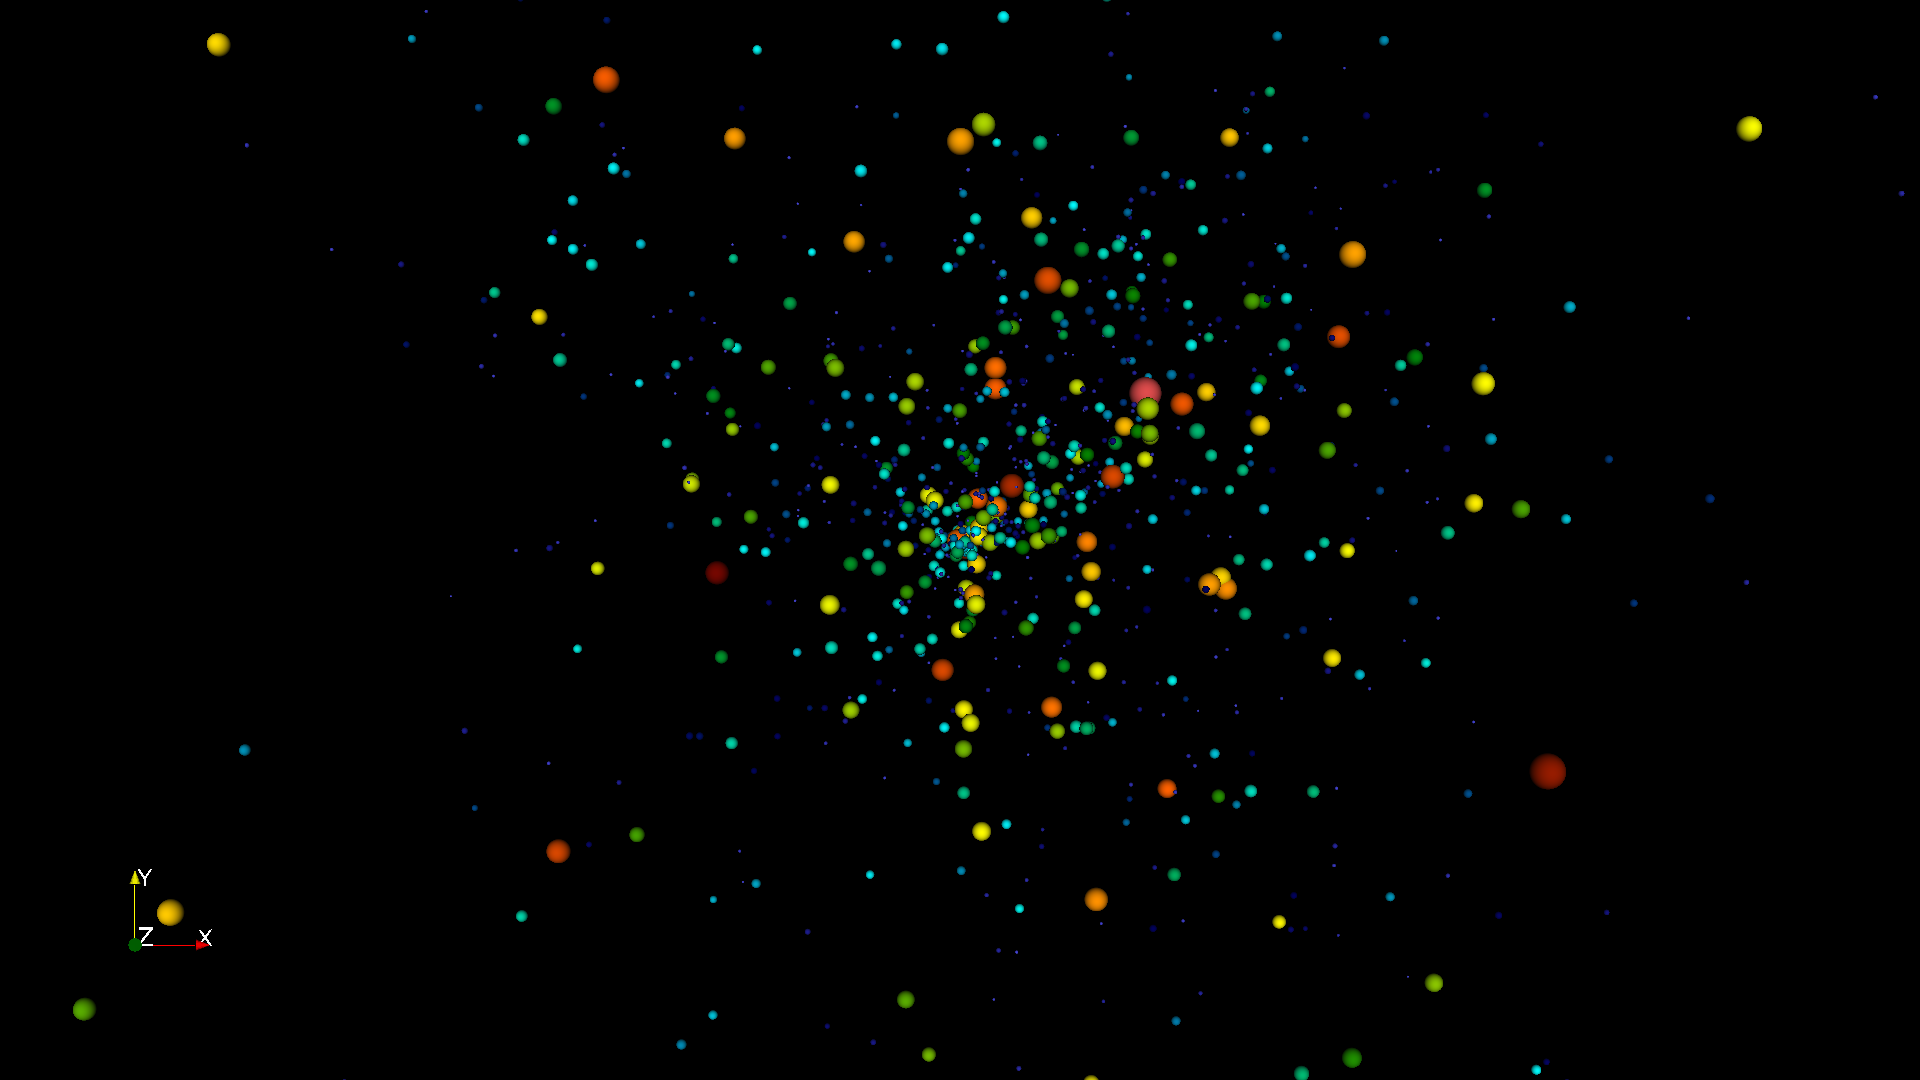
\includegraphics[width=\linewidth]{images/fp/pv-nbody-better}
  \caption{Sample frame from an animation produced from a student's
  simulation using our tool.  The ease of use allowed the student
  to quickly get the tool running, allowing fast and simple visual
  debugging.}
  \label{fig:nbody}
\end{figure}

The flexibility of the system was a boon in this environment.
Visualizing the data in-memory would be difficult. The data were
distributed, and the writes were in ASCII; parsing the data from the
given stream was daunting for undergraduates.  Therefore they elected
to delay launching ParaView until after a timestep completed.  The
system must write and then read particle information from disk, but
visualization was still concurrent with simulation and faster than
serializing the two tasks.  Most importantly, the simplicity allowed
application of the technique in
\textit{tens of minutes}.

% \subsection{Stop the world vs. Asynchronous}
%
% \subsection{In-process vs. Out-of-process}
%
% shared memory vs. just relying on the disk cache
%
% \subsubsection{Out-of-process: launching jobs from within a job}
%
% \subsubsection{Out-of-process advantage over inotify}
%
% it works even over NFS (or other parallel filesystems)

\section{Alternative use cases}
\label{sec:novel}

The ability to hook into \emph{any} data movement operation of a
process enables \freeprocessing{} to create novel applications of
\insitu{} ideas.  In this section, we highlight a couple uses that make
\freeprocessing{} unique among \insitu{} tools.

\subsection{Transfer-based visualization}

A heretofore lost opportunity has been in applying visualization
methods to data \emph{during transport from site to site}.  This use
case shares
the primary motivation behind prior \insitu{} visualization work: that
we should do
operations on data while they are \emph{already} in memory, instead of
writing the data to disk and then reading them back. While most if not
all HPC experts agree that---at the largest scale---moving data will no
longer be viable, a large userbase still exists for which simulation on
a powerful remote supercomputer and analysis on local resources is the
norm.

To downplay this drawback, we propose preprocessing during this transit
time.  As an
example of \freeprocessing{} for this novel case, we use it to
instrument the transfer of a dataset using the popular secure copy
(\texttt{scp}) tool.  The system works by intercepting data as it goes
out to or comes in from a socket.  The source of the secure shell
program itself needs no modification; the system could work with any
network service, such as an FTP client or a web browser.

\begin{figure}
  \centering
  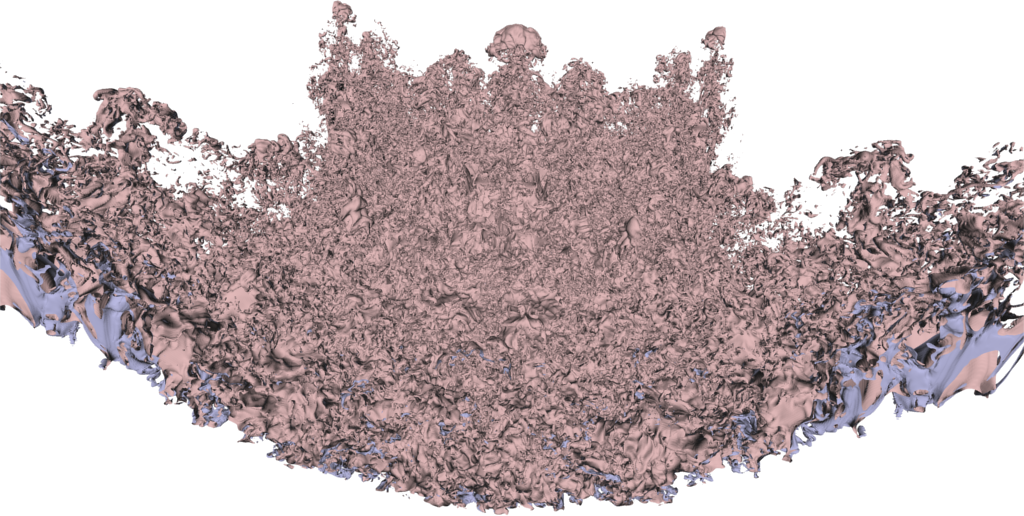
\includegraphics[width=\linewidth]{images/fp/rmeshkov-iso}

  \caption{Richtmyer-Meshkov instability isosurface computed by a
  \freeprocessor{}.  Whereas the \freeprocessor{} could be applied to
  any process that moves data, this particular isosurface was computed
  during network transfer via \texttt{scp}.}

  \label{fig:rm-iso}
\end{figure}

One use case is the computation of an isosurface;
Figure~\ref{fig:rm-iso} shows an example.  A \freeprocessor{} computed
this isosurface of a Richtmyer-Meshkov instability during network
transfer.  This example demonstrates one of the issues with our system:
we needed to modify a marching cubes implementation to work in a
slice-by-slice manner, as opposed to assuming all data were in-core.
Additionally, our marching cubes implementation required at least two
slices to operate, which necessitated a cache in the
\freeprocessor{} to make up for the small writes utilized by
\texttt{scp}.  This buffering and our unoptimized marching cubes
implementation slows down a gigabit-link transfer by 4x.  Although
this still proved faster than transferring the dataset and computing
the isosurface in series, it highlights the pain associated with the
need to rewrite code in a stream processing fashion.  On the other
hand, with the rise of data parallel architectures and the decreasing
memory per core ratio, one might argue that a transition to a stream
processing model is inevitable.

% One example is from GPU volume rendering, which requires data
% organized into regular `bricks' for effective paging.  However, as
% noted by recent
% work~\cite{Fogal:2013:Analysis}, this can become a prohibitively
% expensive operation for suitably large data.  The main cost in data
% reorganization is simply loading and writing the file back to disk;
% moving data around in memory is comparatively fast.
%
% The system works by ... calculating the appropriate new offset, and
% transparently re-routing the data to the bricked position.

\subsection{MATLAB}

% MATLAB is a numerical computing environment.  Though it is not
% typically associated with high-performance computing, it nonetheless
% sees extensive use in engineering domains.  It is therefore impossible
% to change the behavior of the program through conventional means, as
% the commercial software is only distributed in binary form.

Users often request methods to read outputs of binary-only commercial
software in tools like
VisIt.\footnote{c.f. ``Using MATLAB to write Silo files to bring
data into VisIt'', \texttt{visit-users} mailing list, February 2014.}.
We implemented a \freeprocessor{} that accepts raw data, reads a
metadata description from a configuration file for semantics, and
exports these data into a Silo file that VisIt can easily import.
Applying this
\freeprocessor{} incurs an additional overhead of 3--10\% on a simple
Julia set calculation in MATLAB, due to the additional data that it
writes.

The alternative of an `export to Silo' MATLAB extension has notable
drawbacks. First, one must compile using the `\texttt{mex}' compiler
frontend, and every major MATLAB update will require a recompilation or
even rewrite.  Second, divorcing the code from MATLAB and its interface
may require significant effort.
In contrast, our \freeprocessor{} is indendendent of the MATLAB version
it instruments, with neither source changes nor a recompilation
required.
Furthermore, the same \freeprocessor{} is applicable in other manners,
such as creating Silo files during a network transfer.

% \TODO{\subsection{Provenance}}

\section{Conclusions}
\label{sec:fp-conclusion}

In this paper we have introduced \textit{Freeprocessing}: an \insitu{}
visualization and analysis tool based on binary instrumentation.  The
method imbues
an existing simulation with \insitu{} powers, with little or---in
some cases---no effort on the part of the simulation author.  The
method's generality enables novel applications, such as visualization
during network transfer or instrumenting software for which source is
unavailable.

The system is, however, not without its drawbacks.  The symbiont
is stable, but customizing the system via new
\freeprocessor{}s can require per-simulation effort.  Furthermore,
the unidirectional communication model precludes simulation steering
applications.
The ability of \freeprocessing{} to insert small,
\textit{ad hoc} bits of code in myriad new places uncovers perhaps
its greatest limitation: increased programmability requires increased
programming.

The work presented here lowers the barrier of entry for a
simulation to indulge in \insitu{} processing.  Previous work on
\insitu{} has largely focused on achieving highly scalable results,
with less regard to the amount of integration effort required.  The
most significant contribution of this work may be that fruitful
capabilities can arise from a modicum of effort.

%Future work in \freeprocessing{} will center around methods for pulling
%additional metadata from the environment, as well as the
%definition of novel \freeprocessor{}s.
